\section{Проектирование}

В данном разделе будет описан процесс проектирования основных
модулей программного средства.

\subsection{Общее описание серверной архитектуры}
\label{sec:overview}

Главная задача сервера --- предоставить API для работы веб-клиента и, возможно,
приложений на других платформах. Данную задачу эффективно решает архитектурный 
стиль взаимодействия компонентов распределённого приложения REST.

REST представляет собой согласованный набор ограничений, учитываемых при 
проектировании распределённой гипермедиа-системы, такие как отсутсвие состояния, 
единообразие интерфейса, идентификация ресурсов в запросах. 

Разработка приложения с помощью данной архитектуры позволяет добиться расширяемости API,
уменьшении нагрузки на сервер за счёт вынесения большьшинства логики отображения и обработки 
данных на веб-клиент.

Общая структура работы клиент-серверного приложения с ипользованием архитеркуты 
REST представлена на рисунке \ref{fig:rest}.

\begin{figure}[h] 
  \centering  
  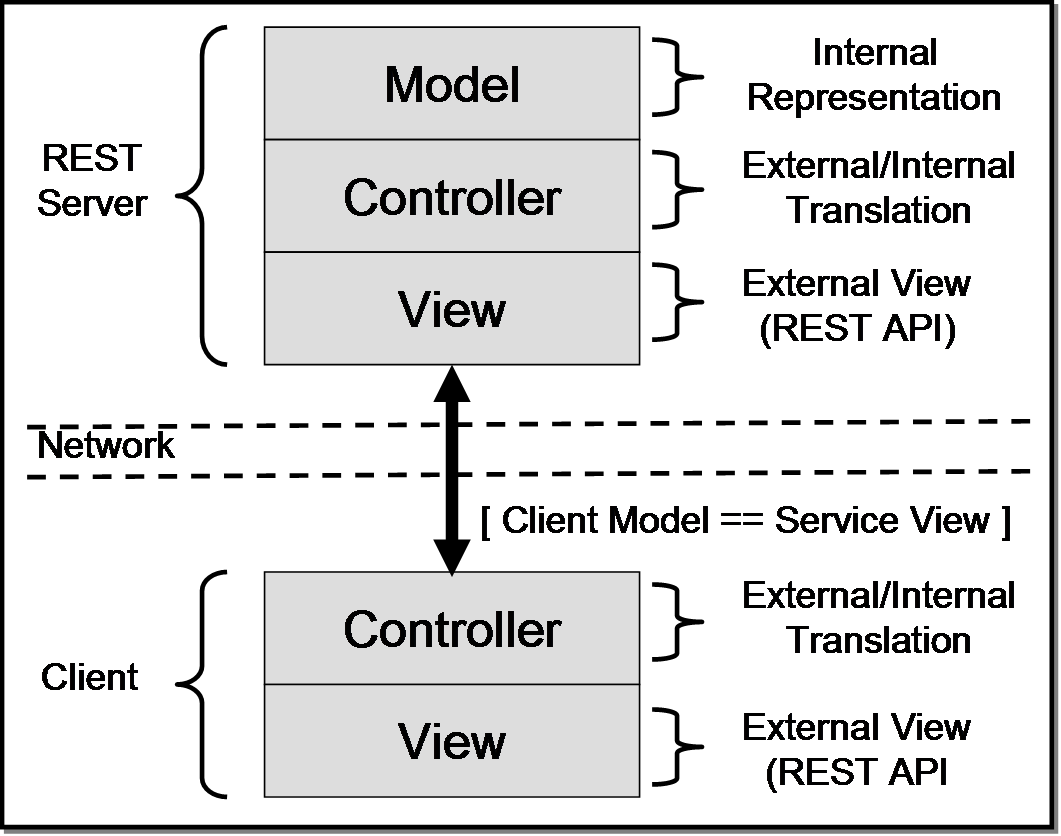
\includegraphics[scale = 0.65]{rest.png}
  \caption{Структура работы клиент-серверного приложения с ипользованием REST архитектуры}
  \label{fig:rest}
\end{figure}

С точки зрения программной архитектуры приложения, было принято решение использовать 
классическую монолитную архитектуру, имеющую следующие слои:

\begin{itemize}
  \item слой контроллеров --- часть сервера, предоставляющая API клиенту и принимающая 
  запросы от него;
  \item слой сервисов --- основная часть серверной части приложения, содержащая бизнес логику 
  приложения, обработку ошибок и работу с базой данных;
  \item слой репозиториев --- абстракция над базой данных, предоставляющая возможности работать с ней 
  остальной части приложения.
\end{itemize}

Приемуществами монолитной архитектуры является скорость разработки, простота, расширяемость. Данная 
архитектура отлично походит для малых и средних приложений, каким и является данный курсовой проект.

\subsection{Функции прогнозирования}
\label{sec:prediction}

Одной из важных особенностей разрабатываемого приложения является функция прогнозирования.

Среди классов методов прогнозирования можно выделить следующие:
\begin{itemize}
  \item методы, основанные на сглаживании, экспотенциальном сглаживании и скользящем среднем;
  \item регрессионные методы прогнозирования;
  \item нейросетевые модели бизнес-прогнозирования.
\end{itemize}

Для реализации функции прогнозирования в рамках предметной области решено остановиться на методах, 
основанных на сглаживании, экспотенциальном сглаживании и скользящем среднем. Данные методы отличаются 
простотой реализации, лёгкостью вычислений и умеренной точностью прогноза, чего вполне достаточно для 
решения поставленных задач.

Самой простой моделью прогнозирования является
\begin{equation} 
Y_{t+1}=Y_t, \label{eq:naive}
\end{equation}
что соответствует предположению, что <<завтра будет как сегодня>>. Она не только не учитывает механизмы, 
определяющие прогнозируемые данные (этот серьезный недостаток вообще свойственен многим статистическим 
методам прогнозирования), но и не защищена от случайных флуктуаций, она не учитывает сезонные колебания и тренды.

Моделью, основанной на простом усреднении является
\begin{equation} 
Y_{t+1}=\frac{1}{T+1}(Y_t+Y_{t-1}+...+Y_{t-T}), \label{eq:avg}
\end{equation}
и в отличии от самой простой модели, описанной уравнением (\ref{eq:naive}), которой соответствовал принцип 
<<завтра будет как сегодня>>, этой модели соответствует принцип <<завтра будет как было в среднем за последнее время>>. 
Такая модель  более устойчива к флуктуациям, поскольку в ней сглаживаются случайные выбросы относительно среднего.

В приведенной выше формуле (\ref{eq:avg}) предполагалось, что ряд усредняется по достаточно длительному 
интервалу времени. Однако? как правило, значения временного ряда из недалекого прошлого лучше описывают 
прогноз, чем более старые значения этого же ряда. Тогда можно использовать для прогнозирования скользящее среднее:
\begin{equation} 
Y_{t+1}=\frac{1}{T+1}(Y_t+Y_{t-1}+...+Y_{t-T}). \label{eq:movavg}
\end{equation}
Смысл его заключается в том, что модель видит только ближайшее прошлое (на T отсчетов по времени в глубину) 
и основываясь только на этих данных строит прогноз.

Метод, описнный в формуле (\ref{eq:movavg}) больше всего подходит для решения задачи, поставленной в данной 
курсовой работе. С его помощью предполагается рассчитывать вероятные расходы пользователя исходя из его последних трат, 
что, в сочетании с средней ежедневной суммой до ближайшей зарплаты позволяет сообщать пользователю о возможной нехватке 
денег в до зарплаты.

\subsection{Разработка API}
\label{sec:api}

API приложения должен позволять пользователю полностью взаимодействовать с приложением и всеми доступными 
ресурсами. Для разработки API требуется выделить сущности приложения, с которыми будет происходит взаимодействие.

В предметной области данного курсового проекта можно выделить следующие сущности:
\begin{itemize}
  \item User --- сущность, представляющая собой самого пользователя системы, хранящая информацию о нём;
  \item Currency --- необходима для поддержки мультивалютности системы, содержит информацию об интернационалом 
  коде валюты и способе корректного отображения с числами;
  \item Wallet --- представляет собой счёт пользователя;
  \item Category --- категория расходов или доходов пользователя, служит для подсчёта статистики трат;
  \item Transaction --- сущность, представляющая собой денежную операцию со счетам пользователя, основная 
  сущность системы.
\end{itemize}

Первоочерёдная задача API --- поддерживать основные CRUD-операции для каждой из этих сущностей. Для сущности 
пользователя необходимо добавить возможности зарегестрироваться и авторизоваться. Также необходимо добавить набор 
необходимых функций для других сущностей. Описание разработанного API приведено в 
таблице \ref{table:api}.
\begin{center}
\begin{longtable}{ 
      | >{\centering}m{0.35\textwidth} 
      | >{\centering}m{0.12\textwidth} 
      | >{\centering\arraybackslash}m{0.45\textwidth}|}
  \caption{Описание API приложения}
  \label{table:api}\\
  \hline Идентификатор ресурса & HTTP \\ метод & Описание\\ \hline
  \endfirsthead
  \caption* {Продолжение таблицы \ref{table:api}}\\
  \hline 
    Идентификатор ресурса & HTTP \\ метод & Описание\\
  \endhead
  \hline
    /api/users/register                        & POST & Регистрация нового пользоватля\\
  \hline
    /api/users/logout                          & POST  & Выход пользователя из приложения\\
  \hline
    /api/users/change-password                 & POST & Смена пароля пользователя\\
  \hline
    \multirow{2}{*}{/api/users/salary-info}    & GET  & Получение информации о зарплате пользователя\\
  \cline{2-3}
                                               & POST & Смена информации о зарплате пользователя\\
  \hline
    /oauth/token & POST & Получение токена авторизации по протоколу OAuth 2.0\\
  \hline
    \multirow{2}{*}{/api/currencies/} & GET    & Получение всех валют в постраничном режиме\\
  \cline{2-3}
                                      & POST   & Создание новой валюты (недоступно обычным пользователям)\\
  \hline
    \multirow{3}{*}{/api/currencies/:id} & GET & Получение валюты с заданным ID\\
  \cline{2-3}                     
                                      & PUT    & Изменение валюты с заданным ID (недоступно обычным пользователям)\\
  \cline{2-3}
                                      & DELETE & Удаление валюты с заданным ID\\
  \hline
    /api/currencies/all               & GET    & Получение всех валют без постраничного режима\\
  \hline
    /api/currencies/code/:code        & GET    & Получение валюты с заданным кодом\\
  \hline
    \multirow{2}{*}{/api/wallets/}    & GET    & Получение всех счетов пользователя в постраничном режиме\\
  \cline{2-3}
                                      & POST   & Создание нового счета\\
  \hline
    \multirow{3}{*}{/api/wallets/:id} & GET    & Получение счета с заданным ID\\
  \cline{2-3}                     
                                      & PUT    & Изменение счета с заданным ID\\
  \cline{2-3}
                                      & DELETE & Удаление счета с заданным ID\\
  \hline
    /api/wallets/:id \\ ?newWallet=:newId & DELETE & Удаление счета с заданным ID и переносом всех связанных с ним транзакций на другой счёт с такой же валютой\\
  \hline
    /api/wallets/all                  & GET    & Получение всех счетов без постраничного режима\\
  \hline
    /api/wallets/forecast             & GET    & Одна из основных функций приложения. Получение прогноза на будущие затраты, средней суммы в день до зарплаты и количества дней до зарплаты\\
  \hline
    \multirow{2}{*}{/api/categories/}    & GET    & Получение всех категорий пользователя в постраничном режиме\\
  \cline{2-3}
                                         & POST   & Создание новой категории\\
  \hline
    \multirow{3}{*}{/api/categories/:id} & GET    & Получение категории с заданным ID\\
  \cline{2-3}                     
                                         & PUT    & Изменение категории с заданным ID\\
  \cline{2-3}
                                         & DELETE & Удаление категории с заданным ID\\
  \hline
    /api/categories/:id \\ ?newCategory=:newId & DELETE & Удаление категории с заданным ID и переносом всех связанных с ним транзакций на другой другую категорию того же типа\\
  \hline
    /api/categories/all                  & GET    & Получение всех категорий без постраничного режима\\
  \hline
    /api/categories/type/:type           & GET    & Получение всех категорий по заданному типу\\
  \hline
    /api/categories/stats/:type/ \\ :currencyCode & GET    & Получение категорий по данному типу со статистикой по данной валюте за всё время\\
  \hline
    /api/categories/stats/:type/\\:currencyCode\\?from=:fromDate\\\&to=:toDate & GET    & Получение категорий по данному типу со статистикой по данной валюте за время в промежутке между fromDate и toDate\\
  \hline
    \multirow{2}{*}{/api/transactions/}    & GET    & Получение всех транзакций пользователя в постраничном режиме, отсортированные в хронологическом порядке, начиная с самых новых\\
  \cline{2-3}
                                           & POST   & Создание новой тразакции\\
  \hline
    \multirow{3}{*}{/api/transactions/:id} & GET    & Получение тразакции с заданным ID\\
  \cline{2-3}                     
                                           & PUT    & Изменение тразакции с заданным ID\\
  \cline{2-3}
                                           & DELETE & Удаление тразакции с заданным ID\\
  \hline
\end{longtable}
\end{center}
